\documentclass[nobib,finnish,oneside,openany,notoc,a4paper]{tufte-book}

\usepackage[finnish]{babel}
\usepackage{parskip}
\usepackage{wrapfig}
\usepackage{graphicx}
\usepackage{placeins}
\usepackage{tabularx}
\usepackage[dvipsnames]{xcolor}
\usepackage[absolute]{textpos}
\usepackage{ifthen}
\usepackage{hyperref}

\definecolor{vihrea}{RGB}{140, 182, 60}

\setlength{\TPHorizModule}{20mm}
\setlength{\TPVertModule}{\TPHorizModule}
\textblockorigin{25mm}{13mm}

\newfontfamily{\spartan}{League Spartan Bold}
\DeclareTextFontCommand{\textspartan}{\spartan}

\geometry{
  left=24.8mm, % left margin
  textwidth=120mm, % main text block
  marginparsep=8.2mm, % gutter between main text block and margin notes
  marginparwidth=35mm % width of margin notes
}

\newcommand{\textls}[2][5]{%
    \begingroup\addfontfeatures{LetterSpace=#1}#2\endgroup
  }
  \renewcommand{\allcapsspacing}[1]{\textls[15]{#1}}
  \renewcommand{\smallcapsspacing}[1]{\textls[10]{#1}}
  \renewcommand{\allcaps}[1]{\textls[15]{\MakeTextUppercase{#1}}}
  \renewcommand{\smallcaps}[1]{\smallcapsspacing{\scshape\MakeTextLowercase{#1}}}
  \renewcommand{\textsc}[1]{\smallcapsspacing{\textsmallcaps{#1}}}
  \usepackage{fontspec}

  \renewcommand{\maketitlepage}[0]{%
  \cleardoublepage%
  {%

  \sffamily%
  \begin{fullwidth}%
    
\includegraphics[width=14cm]{Viite cmyk green.pdf}
  \vspace{8.5pc}%
  \fontsize{32}{50}\spartan{\par\noindent\textcolor{vihrea}{\allcaps{\thanklesstitle}}}
  \vspace{6pc}%
  
  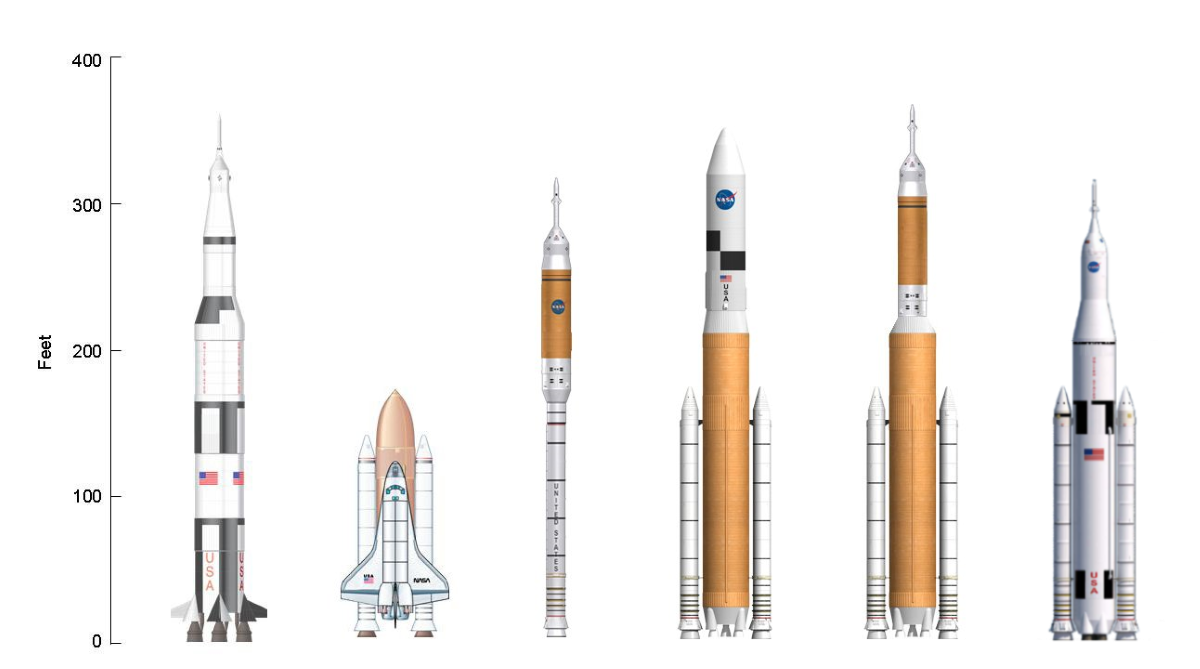
\includegraphics[width=15cm]{etusivu.png}

  \vspace{4pc}%

  \fontsize{8}{16}\selectfont\par\noindent\allcaps{Viite - Tieteen ja teknologian vihreät ry:n avaruuspoliittinen kannanotto\\ \noindent 15.12.2022}%

  \end{fullwidth}%
  }

  \thispagestyle{empty}%
  \clearpage%
}

\title{Suomesta avaruuden edelläkävijä}
\author{Viite - Tieteen ja teknologian vihreät ry}
\publisher{}
\date{3.12.2022}

\begin{document}

\maketitlepage

\chapter{Johdanto}

Avaruus on megatrendi. Avaruusteknologia koskettaa meitä kaikkia
päivittäin. Avaruustutkimuksen ja -tekniikan merkitystä nykyaikaisessa
yhteiskunnassa ei voi ylikorostaa, mutta aiheen poliittinen käsittely on
jäänyt Suomessa sivuosaan.

Avaruuden kestävä käyttö on keskeinen teema resilientissä
yhteiskunnassa. Käynnissä oleva Venäjän hyökkäyssota Ukrainassa on
konkretisoinut avaruusteknologian merkityksen yhteiskunnalle ja
erityisesti puolustussektorille. Avaruusteknologian ratkaisut tulevat
auttamaan meitä selättämään ilmastokriisin ja muita ihmiskunnan
kohtaamia haasteita.

Suuri kiitos kaikille kannanottoa kommentoineille ja sen kirjoittamisessa
auttaneille. Geopoliittinen järjestys on juuri tällä hetkellä valtavien
haasteiden edessä ja tilanne voi kehittyä nopeastikin. Kaikki kannanotossa
esitetyt asiat on esitetty parhaassa tällä hetkellä käytettävissä olevan
tiedon valossa.

\textit{Helsingissä 15.12.2022}

Ville Seppälä, puheenjohtaja

Paavo Heiskanen, projektipäällikkö

Tuomo Liljenbäck, toiminnanjohtaja

Janne Peltola, taitto ja oikoluku

\vspace{5cm}

Tämä julkaisu on jaettavissa Creative Commons CC-BY-SA 4.0-ehdoin.

This publication is released under Creative Commons CC-BY-SA 4.0.

\textbf{An English version is available at the end of the paper. }

\chapter{Taustaa}

Ympäristön suojelu ja kestävä käyttö ei rajoitu ilmakehän sisäpuolelle.
Maapalloa ympäröivän lähiavaruuden käyttäminen taloudellisiin ja
sotilaallisiin tarkoituksiin on monipuolistunut ja lisääntynyt
kuluneiden vuosikymmenien aikoina. Lähiavaruudella tarkoitetaan tässä
yhteydessä sitä avaruuden osaa, jota maapallon magneettikenttä
kontrolloi (ks. Kuva 1). Tämä on avaruuden alue, jossa kaukokartoitus-,
telekommunikaatio-, ja säähavaintosatelliitit toimivat.

Teknologian kehitys ja niin sanotut uuden avaruusteollisuuden yritykset
ovat moninkertaistaneet maapalloa kiertävien satelliittien määrän.
Myöskään avaruuden käyttö sotilaallisiin tarkoituksiin ei ole enää
pelkästään suurvaltojen toimialaa vaan lähes kaikkien valtioiden
saavutettavissa. Lisäksi ei ole poissuljettua, että sotilaallista voimaa
käytettäisiin kaupallisten toimijoiden satelliitteihin, mikäli niiden
koetaan olevan uhka muulle sotilaalliselle toiminnalle. Yhteiskuntamme
ja sen instituutiot ovat tulleet entistä enemmän riippuvaisiksi
avaruusteknologian hyödyntämisestä.

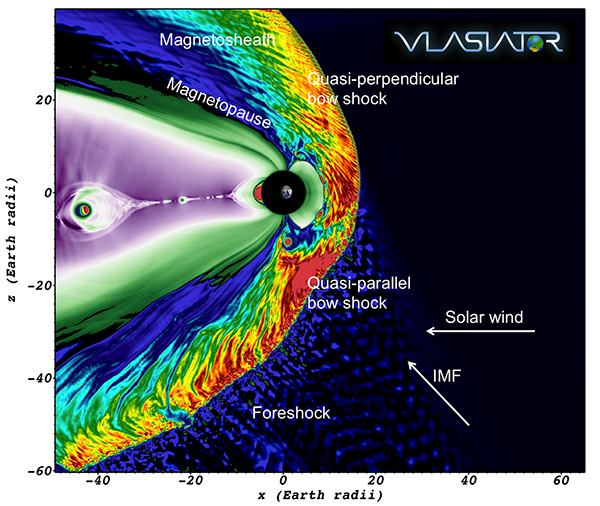
\includegraphics[width=10.5cm]{image1.png}

\emph{Kuva 1 - Magnetosfääri ulottuu
päiväpuolella n.~10 maan säteen päähän, yöpuolella satojen maan säteiden
päähän. Kuvalähde Minna Palmroth / Helsingin Yliopisto}

Lähiavaruudesta on tullut yhä enemmän taloudellisen ja sotilaallisen
toiminnan painopistealue. Muuttunut toimintaympäristö vaatii
lisääntynyttä aloitteellisuutta päätöksentekijöiltä avaruuspolitiikan
uhkiin ja mahdollisuuksiin. Suomi on säätänyt lain avaruustoiminnasta,
joka on hyvä perusta avaruuspolitiikalle {[}1{]} ja tehnyt selvityksen
avaruuden toimintaympäristön muutoksesta {[}2{]}. Lisäksi hallitus on
antanyt esityksen laista kaukokartoituspalveluiden ja maa-asemien
sääntelystä {[}3{]}. Suomessa on hajautettu avaruushallinto
(\href{https://spacefinland.fi/avaruushallinto}{\emph{https://spacefinland.fi/avaruushallinto}})
ja julkaistu avaruusstrategia {[}4{]}. Avaruuden tilannekuva ja
avaruuspuolustus on huomioitu vuoden 2021 puolustusselonteossa {[}5{]}.
Muita toimijoita on kuvattu liitteessä 1.

Avaruuden kestävän käytön {[}6{]} varmistamiseksi on olennaista, että
Suomi osana eurooppalaista ja pohjois-Atlantin yhteisöä käy tarvittavaa
keskustelua nykytilanteen vaatimalla tasolla. Kestävyydessä on otettava
huomioon taloudelliset, yhteiskunnalliset ja ympäristöön liittyvät
näkökulmat (ks. Kuva 2). Vaikka Suomen vaikutusvalta on kansainvälisesti
verrattaen pieni, EU:n ja ESA:n kautta pystymme vaikuttamaan
merkittävällä painoarvolla. Panostukset tutkimukseen, tuotekehitykseen
ja kansainväliseen yhteistyöhön ovat ensiarvoisen tärkeitä. Erityisesti
avaruuteen liittyvä perustutkimus ja siitä lähtöisin olevat
ympäristökeskeiset, yhteiskunnalliset ja taloudelliset näkökulmat on
huomioitava.

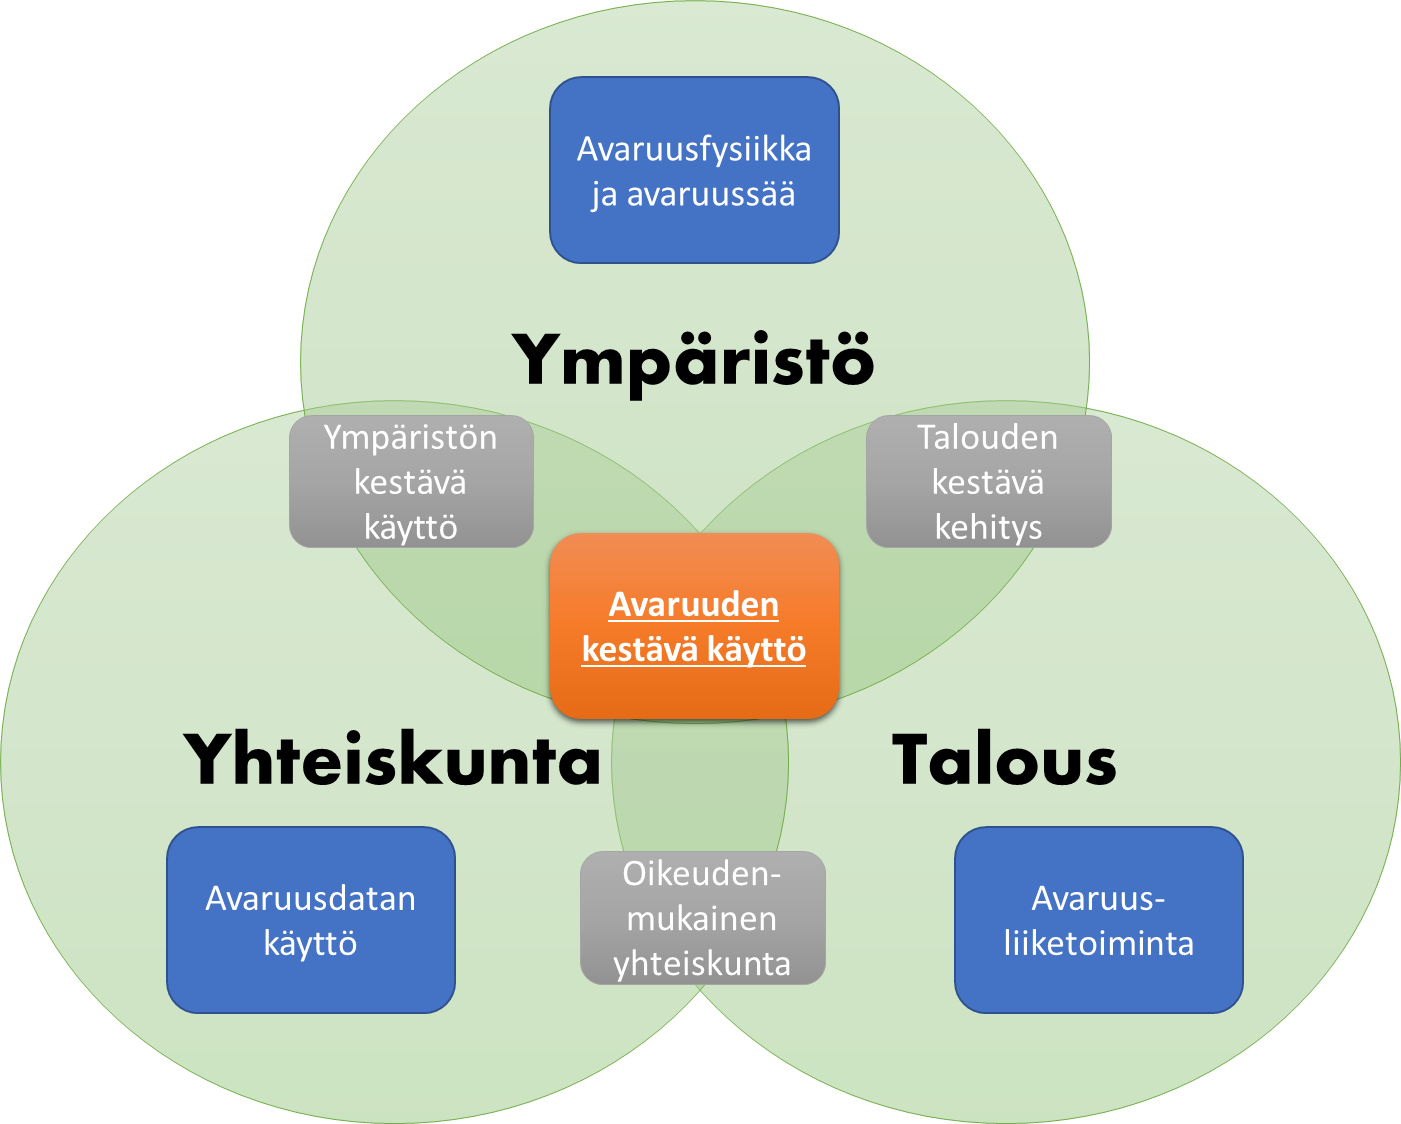
\includegraphics[width=11cm]{image3.png}

\emph{Kuva 2 - Avaruuden kestävä käyttö}

Lähiavaruuden pilaaminen avaruusromulla on estettävä kansainvälisillä
sopimuksilla. Yrityksille ja instituutioille on tarjottava
mahdollisuudet kehittää kestäviä ratkaisuja, jotka mahdollistavat
avaruuden käytön niin, että siitä on mahdollisimman suuri hyöty
mahdollisimman monelle ihmiselle. Suomen täytyy valmistautua
puolustautumaan erilaisia avaruusteknologian käyttöön liittyviä
uhkakuvia vastaan. Erittäin pitkän aikavälin tähtäimenä ihmiskunnalle on
asuttaa muita planeettoja, jotta olemassa oloamme uhkaavat riskit
pienentyvät. Tämä on mahdollista vain, jos sekä elinkelpoisesta
elinkehästä ilmakehän sisäpuolella että avaruuden kestävästä käytöstä
sen ulkopuolella huolehditaan.

Avaruusteknologia tarjoaa valtavia taloudellisia mahdollisuuksia
{[}7-9{]}, joiden hyödyntämiseksi on toimittava viipymättä.
Avaruustoimintaan tulee panostaa merkittävästi resursseja. Nykyisin Työ-
ja Elinkeinoministeriön avaruusosasto edustaa Suomea, mutta ei hallinnoi
rahoitusta kokonaisuutena. Yksi vaihtoehto on, että Suomeen perustetaan
yhtenäinen avaruushallinto valtioneuvoston tasolle, joka koordinoi
kansallisen avaruusstrategian toimeenpanoa ja resursointia.
Avaruushallinnon tulee edustaa Suomea kansainvälisissä ympäristöissä
(ks. Liite 1) ja ylläpitää avaruustutkimuksen rahoituskokonaisuutta,
joka on tällä hetkellä hajautunut monen eri toimijan alueelle.

\chapter{Tavoitetila}

\begin{itemize}
\item Avaruusteknologian avulla tuotettua
tietoa käytetään kokonaisvaltaisesti päätöksenteon tukena.
\item Ilmastopäästöt pystytään paikallistamaan yksittäisen päästölähteiden
tarkkuudella.
\item Luonnonkatastrofeja ja turvallisuusuhkia pystytään
ennakoimaan ja niiden vaikutuksia lieventämään.
\item Valtionhallinnon, virastojen, yritysten ja yliopistojen välillä käydään aktiivista
keskustelua siitä mitä tietoa tarvitaan ja miten se voidaan tehokkaimmin
tuottaa.
\item Suomessa on vahva itsenäinen ja kansainvälisesti hyvin
verkottunut avaruusteollisuus, joka toimii yhteistyössä muiden tahojen
kanssa.
\item Teollisuuden tarvitsevaa työvoimaa koulutetaan aktiivisesti
useissa eri paikoissa, teollisuuden tarpeet huomioon ottaen.
\item Tutkimustoiminta yliopistoissa on vilkasta ja kansainvälistä.
\item Avaruutta ja sen kestävän käytön perusteita opetetaan kouluissa perusopetuksesta
lähtien.
\item Maan hallinto ymmärtää avaruustekniikan sovellusten arvon
määräytymisen perusteet ja tarvittavien toimenpiteiden ja investointien
aikajanan, joka on usein vuosikymmeniä.
\item Avaruuden tuottamaa lisäarvoa mitataan ja arvovirrat on hyvin määritelty ja sisäistetty valtionhallinnossa.
\end{itemize}

\chapter{Lähiavaruuden kestävään käyttöön kohdistuvat uhat}

Vaikka asejärjestelmien testaaminen avaruudessa on vähentynyt kylmän
sodan ajalta {[}10{]}, suurvaltojen kiinnostus avaruuden sotilaalliseen
hyväksikäyttöön on kasvanut. Esimerkiksi Kiinan {[}11{]}, Yhdysvaltojen
{[}12{]}, Intian {[}13{]} ja Venäjän {[}14{]} suorittamat varomattomat
ASAT-testit {[}15{]} lisäävät vaarallisen avaruusromun määrää
lähiavaruudessa. Avaruusromu aiheuttaa turvallisuusuhan avaruuslennoille
ja satelliiteille. YK:lla on päätöslauselma, jonka tarkoituksena on
luoda kansainvälinen normisto avaruudessa tapahtuville sotilaallisille
toimenpiteille {[}16{]}. Yhdysvallat on ollut asiassa aloitteellinen ja
ilmoittanut lopettavansa ASAT-testit, vaatien niiden sääntelyä
kansainvälisellä tasolla {[}17{]}. \textbf{Suomen tulee tuomita jyrkästi
tarpeetonta avaruusromua tuottavat vaaralliset testit. }On myös
pidettävä mielessä että sotilaallinen toiminta avaruudessa ei rajoitu
satelliitteja tuhoaviin asejärjestelmiin, vaan myös muunlainen
vaikuttaminen ja häirintä on mahdollista. Tämä koskee myös kaupallisia
toimijoita joiden satelliitteja tai maa-asemia käytetään sotilaallisen
toiminnan tukemiseen.

Uuden avaruusteollisuuden yritykset ovat edesauttaneet kaupallisen
avaruustoiminnan laajentumista ja mahdollistaneet niin sanottujen
megakonstellaatioiden (tuhansia satelliitteja käsittävät
avaruusjärjestelmät) rakentamisen. Nämä konstellaatiot vaikeuttavat maan
pinnalta suoritettavia tähtitieteellisiä havaintoja {[}18{]} ja lisäävät
vaarallisen avaruusromun määrää. \textbf{Suomen tulee pyrkiä
vaikuttamaan kansainvälisissä järjestöissä niin että konstellaatioihin
kohdistetaan riittävä määrä kansainvälistä sääntelyä haittojen
minimoimiseksi. Sääntelyn ei pidä olla pelkästään rajoittavaa vaan sen
tulisi myös johtaa vaikutusmekanismien ja liiketoimintamahdollisuuksien
syntymiseen. }

Yhä useammat arkipäiväiset toiminnot, kuten satelliittinavigointi,
sääennusteet, ICT, ja kaukokartoitussatelliittien dataa käyttävät
yritykset, ovat riippuvaisia avaruusteknologiasta. Yksi keskeinen
teknologia on navigointijärjestelmien tuottama universaali aikasignaali,
jota käytetään erittäin laajasti ohjaamaan yhteiskunnan elintärkeitä
toimintoja. Avaruusteknologia on kuitenkin haavoittuvaista esimerkiksi
avaruussään aiheuttamille vahingoille. Voimakas avaruusmyrsky {[}19{]}
saattaa aiheuttaa mittavia vahinkoja sekä satelliiteille {[}20{]} että
maanpäälliselle infrastruktuurille. Avaruusmyrskyihin reagointia voidaan
parantaa rakentamalla ja ylläpitämällä avaruussäätä havainnoivia
satelliitteja {[}21{]}. Lisäksi avaruusromu saattaa vaurioittaa tai
tuhota satelliitteja. \textbf{Suomen tulee toimia aktiivisesti
avaruustilannetietoisuuden (SSA {[}22{]}) ja avaruusliikenteen ohjauksen
ja koordinoinnin (STM) kansainvälisen yhteistyön edistämiseksi. Lisäksi
tarvitaan tutkimusrahoitusta, uutta lainsäädäntöä ja viranomaisten
suunnitelmia avaruusmyrskyjen varalle.} Suomi on perustamassa
kansallisen avaruustilannekeskuksen {[}23{]}.

Avaruusturismin suosio on kasvamassa. Uusien, yksityisten
laukaisupalveluiden tarjoajien myötä tämä turismin muoto on siirtymässä
yhä useampien ihmisten ulottuville. Rakettien laukaisuun liittyy
kuitenkin aina suuria päästömääriä ja muita ympäristöhaittoja.
Laukaisulupien myöntäminen on kunkin maan päätäntävallassa.
\textbf{Suomen tulisi kannattaa periaatetta, jossa laukaisujen
ulkoishaitat hinnoitellaan oikein. }

Yksityisten laukaisupalveluiden tarjonta on kasvanut voimakkaasti viime
vuosina. On mahdollista, että osa palveluntarjoajista käyttää ns.
saalistushinnoittelua pyrkien saamaan kilpailua pois markkinoilta
{[}24{]}. On erittäin tärkeää, että eurooppalaisilla yrityksillä,
instituutioilla ja valtioilla on riippumaton pääsy avaruuteen.
Kaupalliset toimijat ovat erittäin kustannustietoisia laukaisupalvelujen
hinnoista, joka tulee merkitsemään tarvetta subventoida itsenäisen
laukaisukapasiteetin aiheuttamat lisäkustannukset yrityksille.
\textbf{Suomen tulee tukea eurooppalaisten laukaisupalvelujen tarjontaa
ESA:n kautta, vaikka tämä tarkoittaisi korkeampia julkisia
laukaisukustannuksia satelliittia kohden. Lisäksi Suomen tulee tukea
uusien eurooppalaisten laukaisupalveluiden tarjoajien
liiketoimintamahdollisuuksia EU:n ja ESA:n kautta. }

Viime aikojen toimitusvaikeudet elektroniikkakomponenttien ja
materiaalien saatavuudessa korostavat riippumattomien toimitusketjujen
tärkeyttä. Suomen tulee toimia aktiivisesti, jotta kriittisiä
komponentteja, materiaaleja ja prosesseja on saatavissa eurooppalaisilta
toimijoilta, jotka täyttävät tiukat ympäristökriteerit. Vaikka
ympäristölainsäädännössä on paljon kehitettävää, Euroopassa on tällä
hetkellä maailman kunnianhimoisin sääntely teollisuuden käyttämille
materiaaleille ja prosesseille. Tiukka ympäristölainsäädäntö tulee nähdä
kilpailutekijänä eurooppalaiselle teollisuudelle ja sitä tulee vahvistaa
ympäristötulleilla materiaaleille, jotka on tuotettu löysemmän
lainsäädännön maissa. \textbf{Eurooppalaisen ympäristölainsäädännön
tulee ottaa huomioon avaruustekniikan erityisvaatimukset ja taata
kriittisten materiaalien saatavuus.}

\chapter{Avaruusteknologian mahdollisuudet}

Suomi on ESA:n ja Euroopan unionin jäsen. Molemmilla on käynnissä
hankkeita, jotka tukevat Suomen kykyä vaikuttaa avaruuspolitiikan
tulevaisuuteen kansainvälisellä tasolla. \textbf{Suomen rahoitusosuutta
ja osallistumista kansainvälisiin avaruushankkeisiin on kasvatettava.}

Avaruusteknologia tuottaa tietoa ilmastokriisiin ja sen vaikutuksiin
liittyen. Panostamalla alan tutkimukseen voidaan varmistaa, että
vaikutuksia selvitetään ja ilmastokriisiin liittyvä päätöksenteko
tehdään parhaaseen mahdolliseen tietoon nojautuen. Tutkimusta ja
koulutusta tehdään tällä hetkellä ainakin Helsingin, Turun ja Vaasan
yliopistoissa sekä Aalto-yliopistossa ja Seinäjoen
Ammattikorkeakoulussa. Avaruusosaamisen on oltava monialaista, sisältäen
esimerkiksi liiketoimintaopetusta, palvelumuotoilua, ja kestävän
kehityksen näkökulmia perinteisen teknologiaosaamisen lisäksi. Lisäksi
on huolehdittava \emph{osaamisen huoltovarmuudesta} teollisessa
toiminnassa, aina ammattikouluista korkeaan opetukseen asti.
\textbf{Tähtitieteen, avaruustieteen ja -teknologian koulutuksen,
tutkimuksen ja tuotekehityksen rahoitusta on lisättävä ja huolehdittava
pätevien ammattilaisten saatavuudesta teollisuuden tarpeisiin.}

Lähiavaruus ja sen tarjoamat mahdollisuudet ovat suurelle osalle
suomalaisista varsin vieraita käsitteitä. Siksi yleistä tietämystä
avaruudesta ja sen hyödyntämisestä tulisi lisätä sisällyttämällä
\textbf{avaruustieteen ja -teknologian opettaminen kansalliseen
opetussuunnitelmaan jo alakoulusta lähtien.} Esimerkiksi Euroopan
avaruusjärjestön alainen ESERO tarjoaa tähän valmiita koulutuspaketteja
ja oppimateriaaleja.

Avaruuden käyttö sotilaallisiin tarkoituksiin on valitettavaa, mutta
väistämätöntä. Yhteiskunnan kriisivalmiuden ja infrastruktuurin
resilienssin kannalta on tärkeää varmistua riittävien valmiuksien ja yhteistyörakenteiden
olemassaolosta. Euroopan unioni tutkii ja kehittää avaruuspuolustuksen
rakenteita ja on julkaisemassa avaruuspuolustusstrategian [25].
\textbf{Puolustusvoimien ja puolustusteollisuuden
kyvykkyyttä avaruustoimintaan osana eurooppalaista ja NATO:n
puolustusyhteistyötä on korostettava.}

Ilmastokriisi tulee aiheuttamaan tuhoisia ympäristöilmiöitä.
Helleaallot, rankkasateet, ja tulvat tulevat vaikuttamaan yhä useampien
ihmisten elämään. Avaruusteknologia tarjoaa mahdollisuudet tutkia ja
ennakoida näitä ilmiöitä ja parantaa yhteiskunnan kykyä reagoida niihin,
eli pelastaa ihmishenkiä ja omaisuutta. {[}26{]} \textbf{Suomen tulee
panostaa satelliittidatan tutkimukseen ja hyväksikäyttöön päätöksenteon
tukena. }

Avaruuden taloudellinen hyväksikäyttö {[}27{]} ei rajoitu pelkästään
kaukokartoitussatelliitteihin ja paikannukseen. Myös tulevaisuuden
teknologiat kuten keskipitkällä aikavälillä realisoituvat kiertoradalla
tapahtuva avaruushuolto (OOS) ja avaruusromun poisto (ADR) tulee ottaa
huomioon. Teollinen valmistus sekä asteroidilouhinta ja mineraalien
kuljetus maapallolle ovat asioita, jotka tulevat päätöksentekoon
pitkällä aikavälillä. Eräät valtiot ovat jo luoneet lainsäädännöllä
toimintaedellytyksiä asteroidien louhinnalle. {[}28{]} Avaruuden käyttö
kaivosteollisuuteen ja valmistukseen saattaa luoda edellytyksiä tuottaa
puhtaan talouden tarvitsemia raaka-aineita ilman maanpäälliseen
kaivosteollisuuteen liittyviä ympäristöongelmia. \textbf{Suomen tulee
luoda liiketoimintaedellytyksiä avaruusteknologian yrityksille, jotka
keskittyvät avaruushuoltoon, avaruusromun poistoon, asteroidilouhintaan
ja kiertoradalla tapahtuvaan valmistukseen.}

Kansainvälisen avaruusasema ISS:n toiminta on nykyrahoituksella
varmistettu vuoteen 2030 asti {[}29{]}. Suomen panos aseman toimintaan
ja ESA:n human spaceflight -ohjelmiin on historiallisesti ollut
vaatimaton. Ihmisten tekemien avaruuslentojen hinta on suuri verrattuna
satelliittien ja robottien suorittamaan tutkimukseen. Lisäksi
panostuksien tuottovaikutus on analysoitava. Kuitenkin vain ihmisten
avaruuslennoilla voimme saada ensikäden tietoa siitä, miten avaruus
ympäristönä vaikuttaa ihmiseen. Lisäksi monimutkaiset kokeet
kiertoradalla vaativat ihmisten läsnäoloa. \textbf{Suomen tulee tutkia
mahdollisuutta osallistua laajemmin ihmisten avaruuslento-ohjelmaan.
}Tätä tukee myös Työ- ja Elinkeinoministeriön tuore raportti {[}30{]}.

Yksityisten rakettien laukaisuja tapahtuu yhä enemmän. Euroopassa
tutkitaan laukaisupaikkoja useissa maissa. Suomi tarjoaa erinomaiset
mahdollisuudet pienten kokeellisten rakettien ampumiseen lähellä
infrastruktuuria Rovajärven ampuma-alueella. \textbf{Suomen tulee tutkia
mahdollisuuksia perustaa laukaisukeskus Rovajärvelle yhteistyössä
puolustusvoimien kanssa, mikäli se on turvallisuusvaatimusten ja
kansainvälisten sopimusten rajoissa ja kansainvälinen
turvallisuusympäristö huomioon ottaen mahdollista. Pohjoismaista
yhteistyötä laukaisupalvelujen suhteen on tiivistettävä.}

Suomessa on aktiivinen avaruusteknologiayritysten ja startupien sekä
kasvuyritysten ekosysteemi. Tätä auttoi merkittävästi alalle räätälöity
New Space Economy-ohjelma (2018-2022) jota hallinnoi Business Finland.
{[}31{]} Laajempi yrityspohja luo uusia liiketoimintamahdollisuuksia ja
vakautta alalle. \textbf{Avaruusteknologiayritysten tutkimus-, kehitys-
ja kansainvälistymisrahoituksen määrää on kasvatettava.}

\chapter{Introduction}


This is a policy paper by The Finnish Greens for Science and
Technology.{\footnote{The Finnish Greens for Science and
  Technology (Viite) is an umbrella association of the Finnish Greens,
  grounded in 2008. The most important goal of the association is to
  advance political decision making that is based on scientific
  knowledge. https://www.viite.fi/english/}

Space is a megatrend. Space technology touches us all every day. The
importance of space research and technology in modern society cannot be
overemphasized, but the political treatment of the topic has remained in
the background in Finland.

The sustainable use of space is a central theme in a resilient society.
The ongoing Russian war of aggression in Ukraine has reinforced the
importance of space technology for humanity and especially for the
defence sector. Moreover, space technology solutions will help us
navigate the climate crisis and other challenges.

Many thanks to everyone who commented on the policy paper and to those
who helped write it. The geopolitical order is facing enormous
challenges, and the situation can develop quickly. Therefore, all
aspects of the program are presented in light of the best currently
available information.


  \chapter{Background}

Environmental protection and sustainable use are not limited to the
interior of the atmosphere. The use of near-Earth space for economic and
military purposes has diversified and increased in the past decades.
Near-Earth space in this policy paper refers to the part of space
controlled by the Earth's magnetic field (see Figure 1). Near-Earth
space is where remote sensing, telecommunications, and weather
observation satellites operate.

Our society and its institutions have become increasingly dependent on
space technology. The development of technology and the so-called new
space industry companies have multiplied the number of satellites
orbiting the Earth. Also, the use of space for military purposes is no
longer only the domain of the great powers but is within reach of almost
all nations. In addition, using military force against satellites of
commercial operators is possible if they are perceived to threaten
military activities.

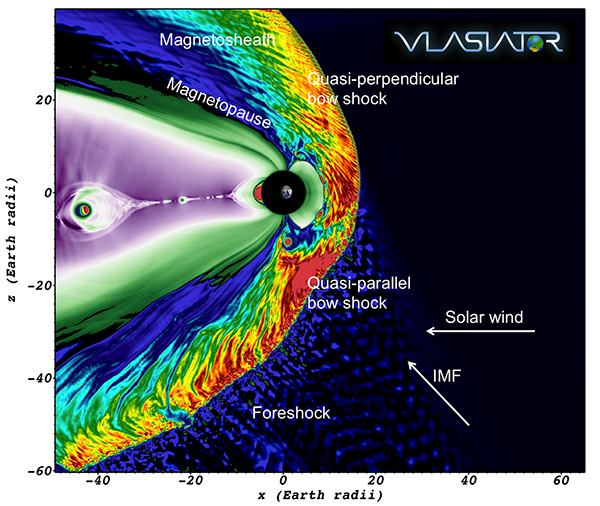
\includegraphics[width=10.5cm]{image1.png}

\emph{Figure 1 - The magnetosphere
extends to about 10 Earth radii during the day and hundreds of Earth
radii during the night. Image source Minna Palmroth / University of
Helsinki}

Near-Earth space has increasingly become a focus area for economic and
military activities. The changing operational environment requires
increased initiative from decision-makers in the threats and
opportunities of space policy. Finland has enacted a law on space
activities, which is a sound basis for space policy {[}1{]} and made a
report on the change in the operating environment of space {[}2{]}. In
addition, the government has presented a law regulating remote sensing
services and ground stations {[}3{]}. Finland has a decentralised space
administration (https://spacefinland.fi/avaruushallinto) and a published
space strategy {[}4{]}. The space situation and space defence have been
taken into account in the 2021 annual defence report {[}5{]}. Other
actors are described in Annex 1.

To ensure the sustainable use of space {[}6{]}, it is essential that
Finland, as part of the European and North Atlantic community, conducts
the necessary discussion at the level required by the current situation.
Furthermore, sustainability must include economic, social and
environmental perspectives (see Figure 2). Although Finland's influence
is small in international comparison, we can significantly influence
through the EU and ESA. Therefore, investments in research, product
development and international cooperation are paramount. In particular,
basic research related to space and its environmental, social and
economic perspectives must be considered.

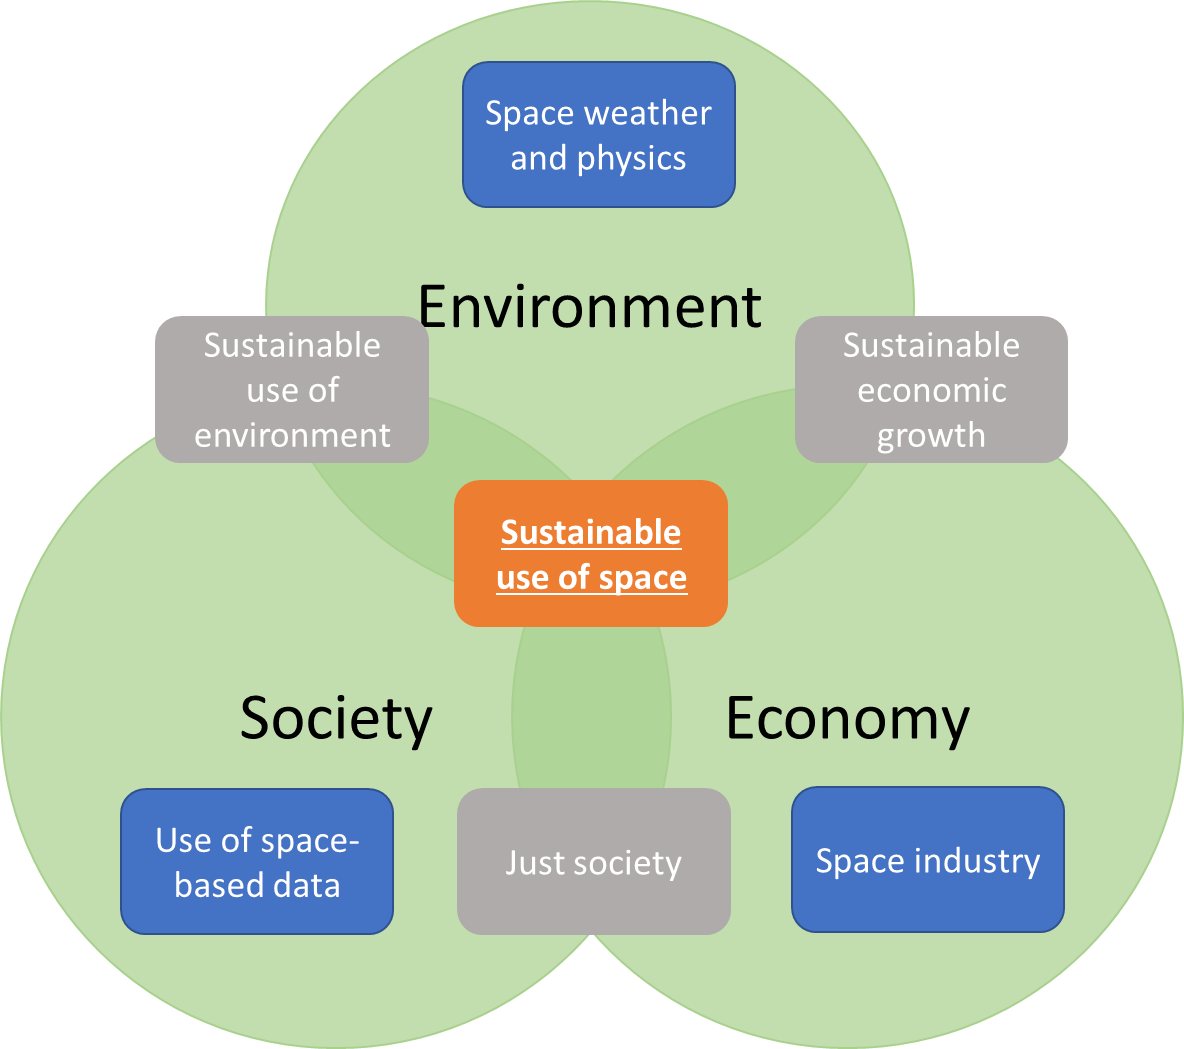
\includegraphics[width=11cm]{image2.png}

\emph{Figure 2 - Sustainable use of space}

Littering near-Earth space with space debris must be prevented by
international agreements. Companies and institutions must be offered
opportunities to develop sustainable solutions that enable the use of
space in such a way that it has the most significant possible benefit
for as many people as possible. Finland must prepare to defend itself
against various threats related to the use of space technology.
Humanity's long-term goal is to inhabit other planets to reduce
existential threats. This ultimate goal is only possible if a viable
life cycle inside the atmosphere and sustainable use of space outside it
are ensured.

Space technology offers enormous economic opportunities {[}7-9{]}, which
must be exploited without delay. Therefore, significant resources must
be invested in space activities. Currently, the Space Department of the
Ministry of Employment and the Economy represents Finland but does not
manage the funding as a whole. One option is for Finland to establish a
unified space administration at the level of the government, which
coordinates the implementation and resourcing of the national space
strategy. The space administration must represent Finland in
international environments (see Annex 1) and maintain the financial
complex of space research, which is currently spread over the territory
of many different actors.

\chapter{Desired Future State}

\begin{itemize}
\item Information produced with the help of space technology is used
holistically to support decision-making.
\item Climate emissions can be
located with the accuracy of individual emission sources.
\item Natural disasters and security threats can be anticipated and their effects
mitigated.
\item There is an active discussion between the state
administration, agencies, companies and universities about what
information is needed and how it can be produced most efficiently.
\item Finland has a strong, independent, internationally well-networked space
industry that cooperates with other stakeholders.
\item The workforce required by the industry is actively trained in several different areas, taking
into account the needs of the industry.
\item Research activities at universities are lively and international.
\item Space and the basics of sustainable use are taught in schools starting from primary education.
\item The country's administration understands the fundamentals of determining the value of space technology
applications and the timeline of actions and investments required, which is often decades-long.
\item The added value produced by the space is measured, and the value flows are well-defined
and internalised in the state administration.
\end{itemize}

\chapter{Threats to the Sustainable use of Near-Earth Space}

Although weapon systems testing in space has decreased since the Cold
War {[}10{]}, the great powers' interest in the military use of space
has grown. For example, careless ASAT tests {[}15{]} by China {[}11{]},
the United States {[}12{]}, India {[}13{]} and Russia {[}14{]} increase
the amount of hazardous space debris in near space. Space debris poses a
security threat to space flights and satellites. The UN has a resolution
that aims to create an international set of norms for military
operations in space {[}16{]}. The United States has taken the initiative
and announced that it would end ASAT tests, demanding their regulation
at the international level {[}17{]}. \textbf{Finland must strongly
condemn dangerous tests that produce unnecessary space debris}. It
should also be remembered that military operations in space are not
limited to weapon systems that destroy satellites. Other types of
influence and interference are also possible. This interference also
applies to commercial operators whose satellites or ground stations are
used to support military operations.

The companies of the new space industry have contributed to the
expansion of commercial space activities and enabled the construction of
so-called mega-constellations (space systems comprising thousands of
satellites). These constellations complicate astronomical observations
from the Earth's surface {[}18{]} and increase the amount of dangerous
space debris.** Finland should strive to influence international
organisations so that a sufficient amount of global regulation is
applied to the constellations to minimise negative externalities.
Regulation should not only be restrictive but also lead to the emergence
of commercial mechanisms and business opportunities.**

More and more everyday activities such as satellite navigation, weather
forecasting, ICT, and companies using data from remote sensing
satellites depend on space technology. One key technology is the
universal time signal produced by navigation systems, widely used to
control society's vital functions. However, space technology is
vulnerable to damage caused by space weather, for example. A powerful
solar storm {[}19{]} could cause extensive damage to both satellites
{[}20{]} and terrestrial infrastructure. The response to space storms
can be improved by building and maintaining space weather observing
satellites {[}21{]}. In addition, space debris may damage or destroy
satellites. \textbf{Therefore, Finland must act actively to promote
international cooperation in space situational awareness (SSA {[}22{]})
and space traffic control and management (STM). In addition, research
funding, new legislation and official plans for solar storms are
needed.} Finland is establishing a national space situation centre
{[}23{]}.

The popularity of space tourism is growing. With new, private launch
service providers, this form of tourism is becoming accessible to more
and more people. However, launching rockets always involves significant
emissions and other environmental harm. The granting of launch permits
is at the discretion of each country.** Finland should support the
principle that the negative externalities of launches are correctly
priced.**

The supply of private launch services has grown enormously in recent
years. Some service providers may use predatory pricing to get
competition out of the market {[}24{]}. European companies, institutions
and states must have independent access to space. Commercial operators
are very cost-conscious about the prices of launch services, which will
mean the need to subsidise the additional costs for companies caused by
independent launch capacity. Finland should support the supply of
European launch services through ESA, even if this means higher public
launch costs per satellite. \textbf{Finland must support the business
opportunities of new European launch service providers through the EU
and ESA.}

The recent difficulties in the availability of electronic components and
materials emphasise the importance of independent supply chains. Finland
must act actively so that critical components, materials and processes
are available from European operators that meet strict environmental
criteria. Although there is much room for improvement in environmental
legislation, Europe currently has the world's most ambitious regulation
for materials and processes used by industry. Strict environmental
legislation should be seen as a competitive factor for European industry
and strengthened by environmental tariffs for materials produced in
countries with looser legislation. In addition, \textbf{European
environmental legislation must consider space technology's particular
requirements and guarantee the availability of critical materials.}

\chapter{The Possibilities of Space Technology}

Finland is a member of the ESA and the European Union. Both have ongoing
projects that support Finland's ability to influence the future of space
policy at the international level. Therefore, \textbf{Finland's
financial contribution and participation in international space projects
must be increased.}

Space technology produces information related to the climate crisis and
its effects. Investing in space research and technology can ensure that
the climate crisis's impact is quantified and that decision-making
related to the situation is made based on the best available
information. Currently, research and education are carried out at least
at the universities of Helsinki, Turku and Vaasa, as well as at Aalto
University and Seinäjoki University of Applied Sciences. Space expertise
must be multidisciplinary, including, for example, business education,
service design, and sustainable development perspectives, in addition to
traditional technology expertise. In addition, care must be taken to
ensure the \emph{availability of competence} in industrial operations,
from vocational schools to higher education. \textbf{Funding for
education, research and product development in astronomy, space science
and technology must be increased, and the availability of qualified
professionals for the needs of the industry must be ensured.}

Near space and the opportunities it offers are foreign concepts to many
Finns. Therefore, general knowledge about space and its utilisation
should be increased by \textbf{including the teaching of space science
and technology in the national curriculum starting from primary school}.
For example, ESERO, under the European Space Agency, offers ready-made
training packages and learning materials.

The use of space for military purposes is unfortunate but inevitable.
In terms of society's crisis preparedness and infrastructure resilience,
it is essential to ensure the existence of sufficient capabilities.
The European Union is studying and developing structures for defence and
space and is drafting an EU space and defence strategy [25]. 
\textbf{The capability of the defence forces and the defence industry
for space operations as part of European and NATO defence cooperation
must be emphasised.}

The climate crisis will cause devastating environmental phenomena. Heat
waves, heavy rains, and floods will affect many people's lives. Space
technology offers opportunities to study and predict these phenomena and
improve society's ability to react to them, i.e.~save lives and
property. {[}26{]} \textbf{Finland should invest in the research and use
of satellite data to support decision-making.}

Economic exploitation of space {[}27{]} is not limited to remote sensing
satellites and positioning. Future technologies such as in-orbit space
servicing (OOS) and space debris removal (ADR), which will be realised
in the medium term, should also be considered. On-orbit manufacturing,
asteroid mining, and transporting minerals to Earth are issues that will
come into decision-making in the long term. Some countries have already
created operating conditions for asteroid mining with legislation.
{[}28{]} Using space for mining and manufacturing may create the
conditions to produce the raw materials needed by a sustainable economy
without the environmental problems associated with surface mining.
\textbf{Finland must create business conditions for space technology
companies focusing on on-orbit maintenance, space debris removal,
asteroid mining and on-orbit manufacturing.}

Current funding ensures the operation of the International Space Station
ISS until 2030 {[}29{]}. Finland's contribution to the station's
operation and ESA's human Spaceflight programs have historically been
modest. The cost of human spaceflight is high compared to research
conducted by satellites and robots. In addition, the return on
investment must be analysed. However, only through human space flights
can we get first-hand information about how space as an environment
affects humans. In addition, complex experiments in orbit require the
presence of humans. \textbf{Finland should investigate the possibility
of participating more actively in the human spaceflight program}. This
approach is also supported by a recent report by the Ministry of Labor
and Economy {[}30{]}.

There are more and more private rocket launches. Launch sites in several
countries are being investigated in Europe. Finland offers excellent
opportunities for firing small experimental rockets close to the
infrastructure at the Rovajärvi firing range.** Finland should explore
the possibilities of establishing a launch centre in Rovajärvi in
\hspace{0pt}\hspace{0pt}cooperation with the defence forces if it is
possible within the limits of security requirements and international
agreements and considering the security environment. Nordic cooperation
regarding launch services must be intensified.**

Finland has an active ecosystem of space technology companies, startups,
and growth companies. The generation of this ecosystem was significantly
assisted by the New Space Economy program (2018-2022), which is tailored
to the sector and is administered by Business Finland. {[}31{]} A
broader business base creates new business opportunities and stability
for the sector. \textbf{The amount of funding for research, development
and internationalisation of space technology companies must be
increased.}

\chapter{Lähteet / References}

\begin{enumerate}
\def\labelenumi{\arabic{enumi}.}
\item
  \href{https://www.finlex.fi/fi/laki/alkup/2018/20180063}{\emph{Laki
  avaruustoiminnasta 63/2018 - Säädökset alkuperäisinä - FINLEX ®}}
\item
  \href{https://julkaisut.valtioneuvosto.fi/bitstream/handle/10024/162062/VNTEAS_2020_08.pdf}{\emph{AVAUS
  -- Avaruuden uuden toimintaympäristön turvallisuusulottuvuudet ja
  liiketoiminta}}
\item
  Hallituksen esitys HE 113/2022 vp
  \href{https://www.eduskunta.fi/FI/vaski/HallituksenEsitys/Sivut/HE_113+2022.aspx}{\emph{HE
  113/2022 vp}}
\item
  Kansallinen avaruusstrategia 2018 -- Työ- ja elinkeinoministeriö\emph{
  }\href{https://tem.fi/documents/1410877/3227301/Avaruusliiketoimintaty\%C3\%B6ryhm\%C3\%A4n+loppuraportti+2018/c6ea3c04-0415-31f5-12ae-dd417d045bed/Avaruusliiketoimintaty\%C3\%B6ryhm\%C3\%A4n+loppuraportti+2018.pdf/Avaruusliiketoimintaty\%C3\%B6ryhm\%C3\%A4n+loppuraportti+2018.pdf?t=1543911842000}{\emph{https://tem.fi/documents/1410877/3227301/Avaruusliiketoimintaty\%C3\%B6ryhm\%C3\%A4n+loppuraportti+2018/c6ea3c04-0415-31f5-12ae-dd417d045bed/Avaruusliiketoimintaty\%C3\%B6ryhm\%C3\%A4n+loppuraportti+2018.pdf/Avaruusliiketoimintaty\%C3\%B6ryhm\%C3\%A4n+loppuraportti+2018.pdf?t=1543911842000}}
\item
  Valtioneuvoston puolustusselonteko 2021
  \href{http://urn.fi/URN:ISBN:978-952-383-820-8}{\emph{Valtioneuvoston
  puolustusselonteko - Valto}}
\item
  \href{https://www.sciencedirect.com/science/article/pii/S0265964621000205}{\emph{Toward
  Sustainable Use of Space: Economic, Technological, and Legal
  Perspectives - ScienceDirect}}
\item
  Measuring the Space Economy: Estimating the Value of Economic
  Activities in and for Space, Institute for Defense Analyses (2020)
  \href{https://www.jstor.org/stable/pdf/resrep25331.7.pdf}{\emph{4.
  Projections of the Future Size of the Space Economy}}, viitattu
  6.10.2022
\item
  \href{https://news.satnews.com/2022/01/27/by-2030-nsr-reports-trillion-in-global-space-economy-revenues/}{\emph{By
  2030, NSR Reports Trillion\$ In Global Space Economy Revenues --
  SatNews}}, viitattu 6.10.2022
\item
  \href{https://www.morganstanley.com/ideas/investing-in-space}{\emph{Investing
  in Space Exploration \textbar{} Morgan Stanley}}, viitattu 6.10.2022
\item
  Ploughshares report: ARMS CONTROL IN OUTER SPACE STATUS, TIMELINE, AND
  ANALYSIS\emph{
  }\href{https://ploughshares.ca/wp-content/uploads/2022/03/ArmsControlOuterSpace_Report.pdf}{\emph{https://ploughshares.ca/wp-content/uploads/2022/03/ArmsControlOuterSpace\_Report.pdf}},
  viitattu 6.10.2022
\item
  \href{https://en.wikipedia.org/wiki/2007_Chinese_anti-satellite_missile_test}{\emph{2007
  Chinese anti-satellite missile test - Wikipedia}}, viitattu 6.10.2022
\item
  \href{https://en.wikipedia.org/wiki/Operation_Burnt_Frost}{\emph{Operation
  Burnt Frost - Wikipedia}}, viitattu 6.10.2022
\item
  \href{https://en.wikipedia.org/wiki/Mission_Shakti}{\emph{Mission
  Shakti - Wikipedia}}, viitattu 6.10.2022
\item
  \href{https://en.wikipedia.org/wiki/Kosmos_1408}{\emph{Kosmos 1408 -
  Wikipedia}}, viitattu 6.10.2022
\item
  \href{https://en.wikipedia.org/wiki/Anti-satellite_weapon}{\emph{Anti-satellite
  weapon - Wikipedia}}, viitattu 6.10.2022
\item
    *\href{https://www.un.org/disarmament/topics/outerspace-sg-report-outer-space-2021/}{\emph{Report
    of the Secretary-General on reducing space threats through norms,
    rules and principles of responsible behaviors (2021)}}
\item
  \href{https://www.cnbc.com/2022/04/18/us-to-end-anti-satellite-asat-testing-calls-for-global-agreement.html}{\emph{U.S.
  commits to ending anti-satellite missile testing, calls for global
  agreement}}, CNBC 18.4.2022, viitattu 6.10.2022
\item
  \href{https://www.nature.com/articles/d41586-021-01954-4}{\emph{Astronomers
  push for global debate on giant satellite swarms}}, Nature, 16.7.2021
\item
    *\href{https://www.mustread.fi/artikkelit/aarimmainen-avaruusmyrsky-voi-iskea-lahitulevaisuudessa-silti-paattajat-eivat-ole-varautuneet-globaaliin-uhkaan/}{\emph{``Äärimmäinen
    avaruusmyrsky voi iskeä lähitulevaisuudessa'' -- silti päättäjät
    eivät ole varautuneet globaaliin uhkaan -- MustRead}}, Minna
    Palmroth 2022,
\item
  \href{https://www.smithsonianmag.com/smart-news/solar-storm-knocks-40-spacex-satellites-out-of-orbit-180979566/}{\emph{Solar
  Storm Knocks 40 SpaceX Satellites Out of Orbit \textbar{} Smart
  News\textbar{} Smithsonian Magazine}} 14.2.2022, viitattu 6.10.2022
\item
  \href{https://kuvaspace.com/2019/06/04/introducing-our-latest-mission-sunstorm/}{\emph{Introducing
  our latest mission: SUNSTORM - Kuva Space}}, viitattu 6.10.2022
\item
  \href{https://www.esa.int/About_Us/ESAC/Space_Situational_Awareness_-_SSA}{\emph{ESA
  - Space Situational Awareness - SSA}}, viitattu 6.10.2022
\item
  \href{https://valtioneuvosto.fi/hanke?tunnus=LVM035:00/2022}{\emph{Avaruustilannekeskuksen
  ohjausryhmä}}, viitattu 1.11.2022
\item
  \href{https://www.ft.com/content/7d561078-37c7-4902-a094-637b81a26241}{\emph{Elon
  Musk being allowed to `make the rules' in space, ESA chief warns
  \textbar{} Financial Times}}, viitattu 6.10.2022
\item
  \href{The Strategic Compass and  EU space-based defence capabilities}\emph{Policy
  Department for External Relations, Directorate General for External Policies of the
  Union. Euroopan parlamentti, marraskuu 2022}
\item
  \href{https://vision.esa.int/rapid-and-resilient-crisis-response/}{\emph{Rapid
  and resilient crisis response -- ESA Vision}}, viitattu 6.10.2022
\item
  \emph{June 2021
  }\href{https://brycetech.com/reports/report-documents/SIA_SSIR_2021.pdf}{\emph{State
  of the Satellite Industry Report}}, Brycetech, viitattu 6.10.2022
\item
  \href{https://miningglobal.com/supply-chain-and-operations/space-race-luxembourg-aims-be-leader-asteroid-mining}{\emph{Space
  race: Luxembourg aims to be leader in asteroid mining}}, viitattu
  6.10.2022
\item
  \href{https://blogs.nasa.gov/spacestation/2021/12/31/biden-harris-administration-extends-space-station-operations-through-2030/}{\emph{Biden-Harris
  Administration Extends Space Station Operations Through 2030}},
  viitattu 6.10.2022
\item
  \href{https://urn.fi/URN:ISBN:978-952-327-704-5}{\emph{Suomen
  osallistuminen Euroopan avaruusjärjestön miehitettyjen avaruuslentojen
  ja avaruuden tutkimuksen ohjelmaan : Selvitys taloudellisista ja
  yhteiskunnallisista hyödyistä - Valto}}, viitattu 6.10.2022
\item
  \href{https://www.businessfinland.fi/en/for-finnish-customers/services/programs/new-space-economy}{\emph{New
  Space Economy program - Business Finland}}, viitattu 6.10.2022
\end{enumerate}

\chapter{Liite 1 - Kansainväliset toimijat avaruuspolitiikassa}

\textbf{Euroopan Avaruusjärjestö (ESA) -
}\href{http://www.esa.int}{\textbf{\emph{www.esa.int}}}

Euroopan Avaruusjärjestö on on kansainvälinen avaruusjärjestö, joka on
perustettu vuonna 1975. Siihen kuuluu 22 jäsenmaata. Suomi liittyi
jäseneksi 1995. ESA on perustamiskirjansa\footnote{https://esamultimedia.esa.int/multimedia/publications/SP-1337/SP-1337\_EN.pdf}
mukaan perustettu vahvistamaan eurooppalaista yhteistyötä avaruuden
tutkimus- ja kehitystyötä puhtaasti rauhanomaisiin tarkoituksiin. ESA on
jaettu direktoraatteihin jotka hallinnoivat eri avaruustutkimuksen
osa-alueita kuten avaruusteknologiaa, kaukokartoitusta,
telekommunikaatiota ja sovelluksia, laukaisupalveluita ja
avaruustiedettä.

\textbf{Euroopan unionin avaruusohjelmavirasto (EUSPA) -
}\href{https://www.euspa.europa.eu/}{\textbf{\emph{https://www.euspa.europa.eu/}}}

Euroopan unionin avaruusohjelmavirasto on perustamisvaiheessa oleva
järjestö, joka toteuttaa Euroopan Unionin avaruusohjelmaa ja tuottaa
avaruuteen liittyviä palveluita. Lisäksi EUSPA tukee tutkimusta ja
innovointia. EUSPA hallinnoi mm. paikannustietopalveluja tuottavia
Galileo- ja EGNOS-palveluita, maaseurantapalvelu Copernicusta ja
satelliittiviestintäojelma GOVSATCOMia.

\textbf{Yhdistyneiden Kansakuntien Avaruusasioiden Toimisto (UNOOSA) -
}\href{https://www.unoosa.org/}{\textbf{\emph{https://www.unoosa.org/}}}**
**

UNOOSA hallinnoi avaruusalan korkeimman tason kansainvälisiä sopimuksia.

\textbf{Kansainvälinen televiestintäliitto (ITU) -
}\href{https://www.itu.int/en/Pages/default.aspx}{\textbf{\emph{https://www.itu.int/en/Pages/default.aspx}}}

Kansainvälinen televiestintäliitto hallinnoi satelliittien
kommunikaatiotaajuus- ja kiertorataparametrien hyväksyntää
kansainvälisesti.

\protect\hypertarget{anchor-17}{}{}Annex 1 - International actors in
space

\textbf{European Space Agency (ESA)} -
\href{http://www.esa.int}{\emph{www.esa.int}}

The European Space Agency is an international space organization that
was founded in 1975. It includes 22 member countries. Finland became a
member in 1995. According to its charter \footnote{https://esamultimedia.esa.int/multimedia/publications/SP-1337/SP-1337\_EN.pdf},
ESA was established to strengthen European cooperation in space research
and development for purely peaceful purposes. ESA is divided into
directorates that manage different areas of space research such as space
technology, remote sensing, telecommunications and applications, launch
services and space science.

\textbf{European Union Space Program Agency (EUSPA)} -
\href{https://www.euspa.europa.eu/}{\emph{https://www.euspa.europa.eu/}}

The European Union Space Program Agency is an organization in the
establishment phase that implements the European Union's space program
and produces space-related services. In addition, EUSPA supports
research and innovation. EUSPA manages e.g.~the Galileo and EGNOS
services that produce positioning information services, the Earth
observation service Copernicus and the satellite communication program
GOVSATCOM.

\textbf{United Nations Office for Outer Space Affairs (UNOOSA)} -
\href{https://www.unoosa.org/}{\emph{https://www.unoosa.org/}}

UNOOSA manages the highest level international treaties in the space
industry.

\textbf{International Telecommunication Union (ITU)} -
\href{https://www.itu.int/en/Pages/default.aspx}{\emph{https://www.itu.int/en/Pages/default.aspx}}

The International Telecommunication Union manages the international
coordination of communication frequencies and orbit parameters for
satellites.
\end{document}